\renewcommand{\theauthor}{Dario Wagner}
\section{Technologien}
\label{sec:Technologien}
\subsection{Allgemeines}
\label{sec:TechnologieAllgemeines}
Die, während der Diplomarbeit, verwendeten Technologien werden anschließend, unter entsprechender Überschrift, beschrieben, wobei auf die wichtigsten, oder auch meist benutzten, genauer eingegangen wird, in Form einer Installation und einer erweiterten Beschreibung. Zudem werden auch alle Technologien beschrieben welche sich nicht bis zum Ende der Arbeit durchsetzen konnten und während der Arbeit auf eine andere gewechselt wurde oder diese überhaupt nicht mehr verwendet wurde. Dies wird jedoch im Beschreibungstext kenntlich gemacht.
\subsection{Programmierung}
\label{sec:TechnologieProgrammierung}
\subsubsection {Visual Studio 17 Community}
\label{sec:VisualStudio17Community}
Visual Studio ist eine Entwicklungsumgebung, für verschiedenste Programmiersprachen, der Firma Microsoft. Die Version 15 / 2017 ist die aktuellste Version und bietet neue Funktionen und Verbesserungen. Unter anderem die voll umfängliche Unterstützung der ASP.NET Core und .NET Core Entwicklung. Die aktuelle Version unterstützt folgende Sprachen:
\begin{itemize}
\item Visual Basic .NET
\item C
\item C++
\item C\#
\item F\#
\item Typescript
\item Python
\item HTML
\item JavaScript
\item CSS
\end{itemize}

Da der Hauptteil der Diplomarbeit in der Objekt Orientierten Programmiersprache C\# geschrieben wurde, hat das Entwicklungsteam Visual Studio 2017 Community verwendet. Hierbei war es wichtig, dass jedes Mitglied der Diplomarbeitsgruppe die selbe "Jahres-Version", in diesem Fall 2017, verwendet, da es zwischen den Versionen kleine Unterscheide, welche zu einem Problem führen könnten, gibt. Ein gravierender Unterschied wäre die Syntax eines Propertys zwischen Version 2013 und 2017. 

\begin{lstlisting}[caption=Syntax Unterschied: Property , label=lst:test]
// Visual Studio 2013 Code
  private string m_Beispiel;
  public string Beispiel
  {
      get { return m_Beispiel; }
      set { m_Beispiel = value; }
  }

// Visual Studio 2017 Code
  private string m_Beispiel;
  public string Beispiel
  {
      get => m_Beispiel;
      set => m_Beispiel = value;
  }
\end{lstlisting}

\subsubsection {.NET Framework 4.6}
\label{sec:.NETFramework4.6}
Am Anfang der Diplomarbeit wurde mit der Firma im Laufe eines Meetings festgelegt, dass bei der Entwicklung des Webservices .net Framework 4.6 verwendet werden soll um die Kompatibilät mit ihren .net Projekten zu garantieren.

Das .NET Framework ist ein Software Entwicklungs-Framework der Firma Microsoft, um Software zu entwicklen, installieren und auszuführen auf Windows basierenden Systemen. 
Aktuell auswählbare Versionen in Visual Studio 2017:\\ 

\centering 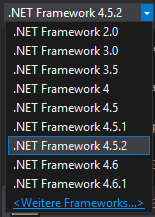
\includegraphics{Technologien_dotNetVersions}

\justifying
\subsubsection {asp.net}
\label{sec:asp.net}
Da das Ziel der Diplomarbeit ein Webservice unter C\# ist, wurde ASP.NET verwendet. ASP.NET ist Teil des .net Framework, mit ihm lassen sich Webservices oder auch Webanwendungen einfach entwickeln. ASP.NET kommt bei 11.8\% aller aktiven Webseiten zum Einsatz und befindet sich deshalb auf dem 2ten Platz nach der Programmiersprache PHP. 
\url {https://w3techs.com/technologies/overview/programming_language/all} 
% DAS DER LINK SO DRIN IS IS NUR VORÜBERGEHEND DAMIT I MA DIE SEITE "MERK"
\\
Im Anschluss wird durch Screenshots erläutert wie ein ASP.NET Projekt in Visual Studio 2017 erstellt wird.

\begin{figure}[H]
    \centering
    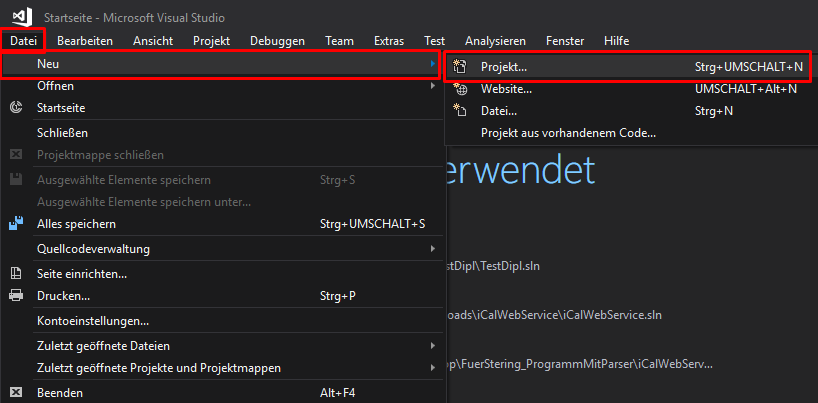
\includegraphics[width=\textwidth]{Technologien_aspNetTutorial01}
    \caption{ASP.NET Projekt erstellen}
    \label{fig:aspNetTut01}

    \centering
    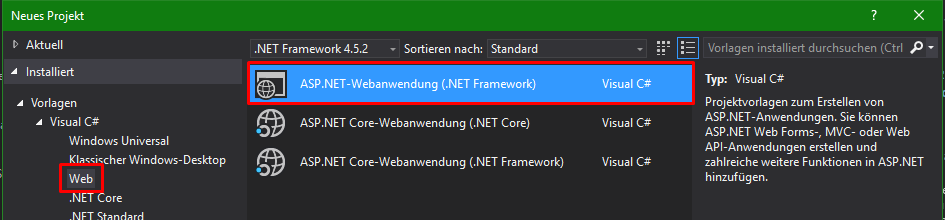
\includegraphics[width=\textwidth]{Technologien_aspNetTutorial02}
    \caption{ASP.NET Webanwendung auswählen}
    \label{fig:aspNetTut02}
\end{figure}
\begin{figure}[H]
    \centering
    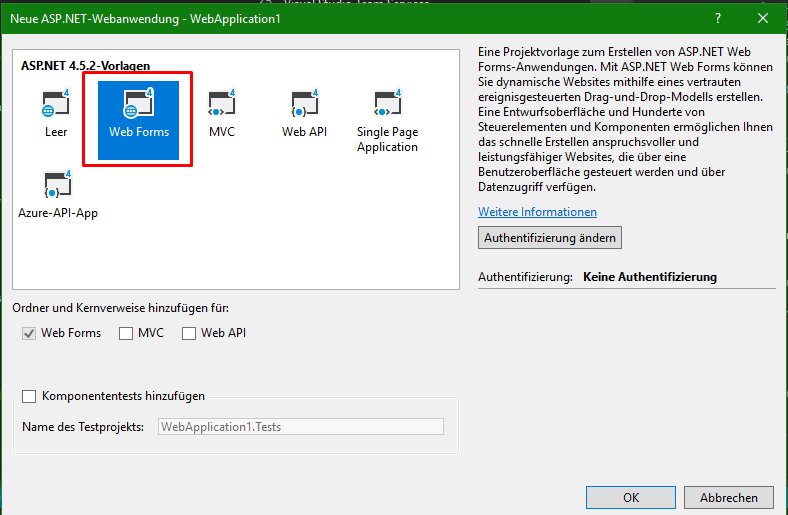
\includegraphics[width=\textwidth]{Technologien_aspNetTutorial03}
    \caption{ASP.NET Vorlage auswählen}
    \label{fig:aspNetTut03}

    \centering
    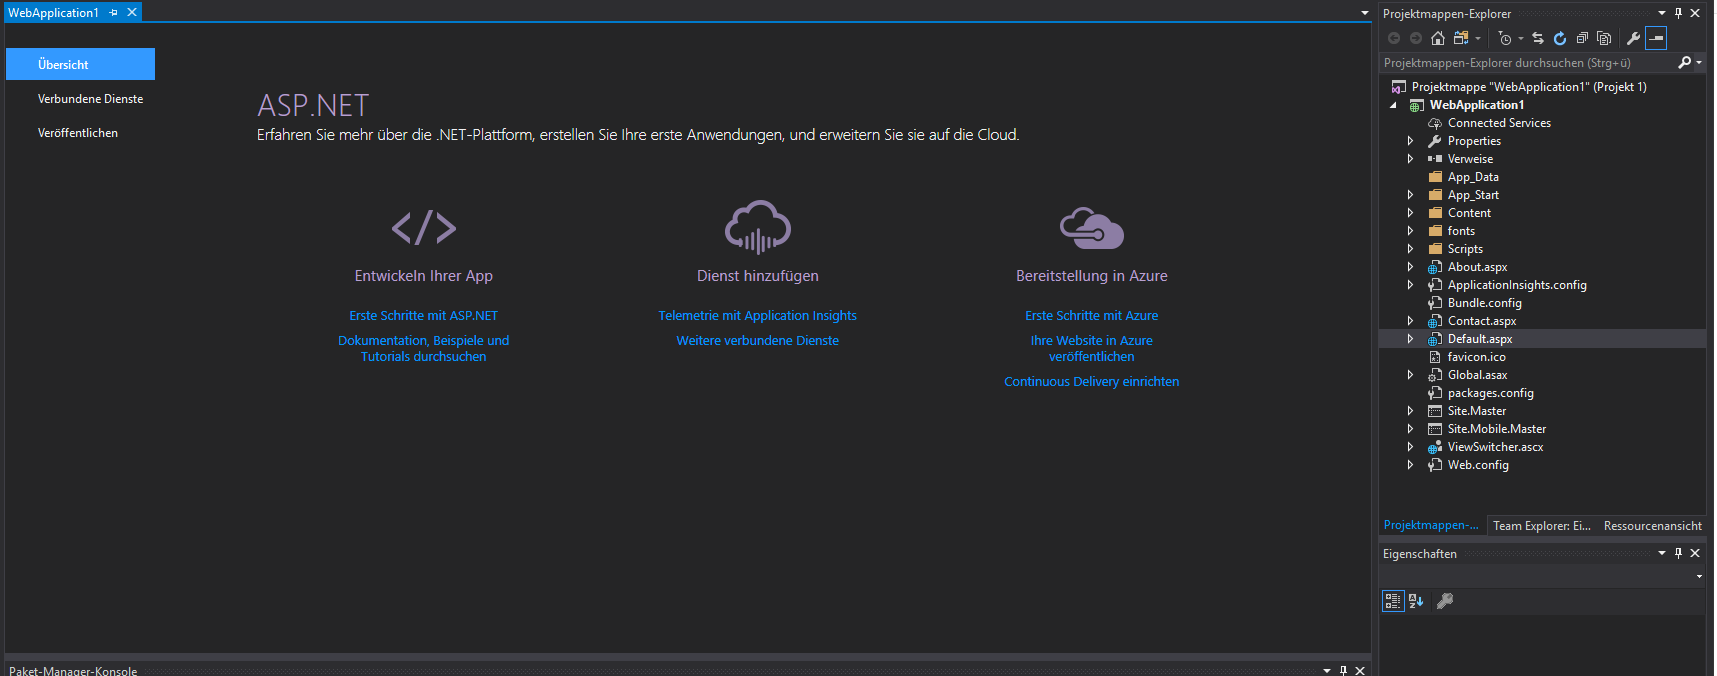
\includegraphics[width=\textwidth]{Technologien_aspNetTutorial04}
    \caption{ASP.NET Projekt Resultat}
    \label{fig:aspNetTut04}
\end{figure}

\subsubsection {MSSQL}
\label{sec:MSSQL}
MSSQL ist KEIN Teil der finalen Diplomarbeit und wurde nur zu Testzwecken verwendet. Im Laufe der Entwicklung wurde von Teammitglied Matthias Franz und Marcel Stering ein Raspberry PI als Datenbank aufgesetzt um einige Tests durchzuführen. Dies wurde mit Microsoft SQL Server verwirklicht. 
\subsubsection {Microsoft SQL Server management Studios}
\label{sec:VisualStudio17Community}
Bei der Microsoft SQL Server entwicklung kam Microsoft SQL Server management Studios zum Einsatz, die Aufgabe des Management Studios war es den Server zu konfigurieren und zu verwalten. 
\subsubsection {Entity Framework}
\label{sec:VisualStudio17Community}
Das Entity Framework ist ein Großteil des Projektparts "Parser" gewesen. Das Entity Framework wird angewandt um den Zugriff auf die Datenbank zu erleichtern. Es dient zur objektrationalen Abbildung auf .NET Objektstrukturen. Auf die Funktionsweise des EFs wird im Parser genauer eingegangen.

\subsubsection {iCal}
\label{sec:VisualStudio17Community}
iCal ist das Format in dem ein Kalender gespeichert wird. Das Format wird unter einer eigenen Überschrift im Laufe der schriftlichen Arbeit genauer erklärt. 
Ein Beispiel für den Aufbau des iCal-Formats sieht wie folgt aus: 
\begin{flushleft}
BEGIN:VCALENDAR \break
   PRODID:-//ACME/DesktopCalendar//EN \break
   METHOD:REQUEST \break
   VERSION:2.0 \break
   BEGIN:VEVENT \break
   ORGANIZER:mailto:sman@netscape.com \break
   ATTENDEE;ROLE=CHAIR;ATTSTAT=ACCEPTED:mailto:sman@netscape.com \break
   ATTENDEE;RSVP=YES:mailto:stevesil@microsoft.com \break
   DTSTAMP:19970611T190000Z \break
   DTSTART:19970701T210000Z \break
   DTEND:19970701T230000Z \break
   SUMMARY:Phone Conference \break
   DESCRIPTION:Please review the attached document. \break
   UID:calsvr.example.com-873970198738777 \break
   ATTACH:ftp://ftp.bar.com/pub/docs/foo.doc \break
   STATUS:CONFIRMED \break
   END:VEVENT
\end{flushleft}
\cite{TechnologieiCalExample}
% WIRD VERÄNDERT WEIL DES MOMENTAN 1 ZU 1 WIKIPEDIA IS
\justifying
\subsubsection {ReSharper}
\label{sec:VisualStudio17Community}
ReSharper ist eine von JetBrains produzierte Erweiterung für Visual Studio, welche das Entwickeln im .NET Bereich erleichtert. Die tschechische Firma JetBrains ist unter anderem Herausgeber von PyCharm, IntelliJ IDEA,  CLion und vielen weiteren hilfreichen Entwicklungs-Tools.

\paragraph {Resharper Installation}
\label{sec:ResharperInstallation}
1. ReSharper auf der JetBrains Seite unter folgendem Link herunterladen: \break \url {https://www.jetbrains.com/resharper/download/} \\
2. Nach Download, die .exe Datei ausführen \\
3. Installierte Visual Studio Version auswählen, License Agreement akzeptieren, anschließend bei gewolltem Paket auf "Install" klicken und auf "Next". 
Wenn man nun auf "Next" geklickt hat werden alle zu installierenden Pakete nochmal angezeigt. Falls die Auswahl passt, auf "Install" klicken. \\
4. Wenn die Installation abgeschlossen ist Fenster schließen. \\
5. Um sicherzugehen, dass die Installation erfolgt ist, Visual Studio starten. Hier sollte nun ein Fenster aufploppen um das Shortcut Sheme auszuwählen.
Wählt man nun eines der Möglichkeiten aus und klickt sich durch Agreements sollte anschließend eine License Information zu sehen sein. Hier beim Paket auf ''Start Evaluation'' klicken und anschließend auf ''OK'' drücken und ReShaper ist funktionsfähig und läuft.

\subsubsection {PostMan}
\label{sec:PostMan}
PostMan wird verwendet um API Tests durchzuführen. Die Software bietet eine sehr übersichtliche Benutzeroberfläche und ermöglicht es dem Benutzer einfach HTTP Requests zu generieren und erspart dem Benutzer große Mengen an Code zu schreiben.\break
\textcite{TechnologiePostman} \\ \break
Man kann zum Beispiel normale GET-Requests senden, bei der Response kann man unter anderem angeben wie sie angezeigt werden soll. Auf der linken Seite sieht man auch eine zeitliche Protokollierung wann welche Anfragen gesendet wurden.

\begin{figure}[H]
    \centering
    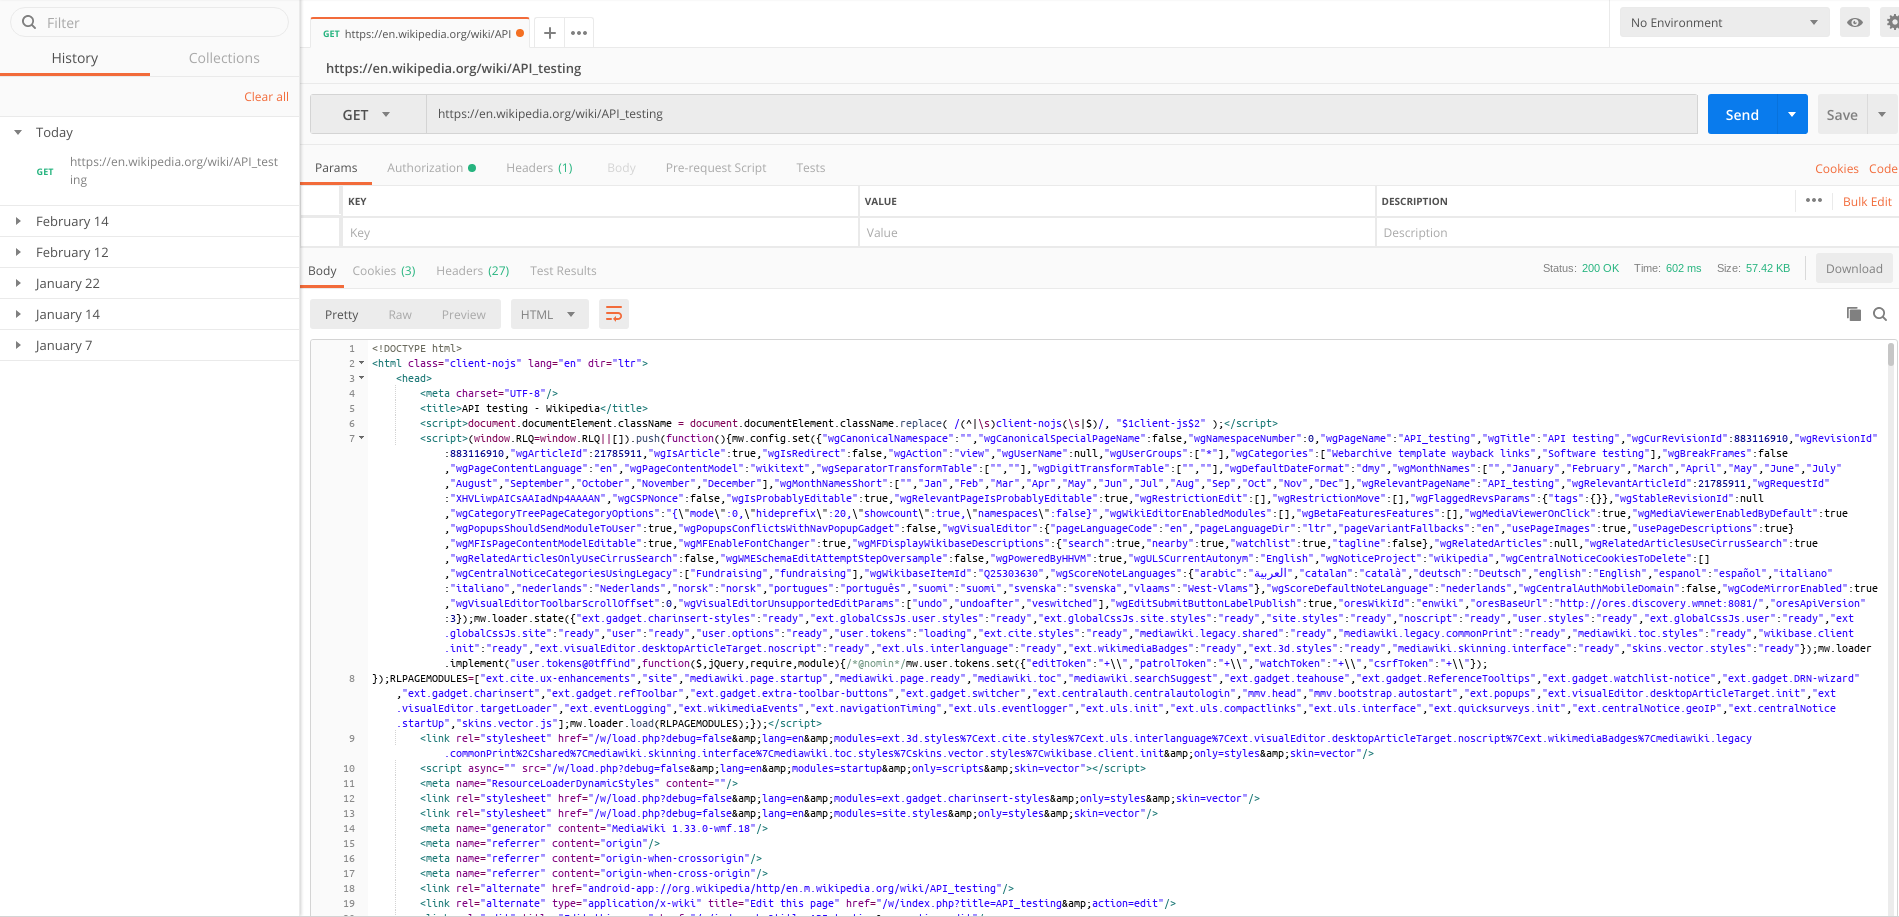
\includegraphics[width=\textwidth]
    {Technologien_Postman01}
    \caption{Postman GET Request}
    \label{fig:Postman}
\end{figure}

Unter dem Tab ''AUTH'' die ''standard authentifications'' setzen. Dadurch kann Postman sich bei einer Request anmelden.

\begin{figure}[H]
    \centering
    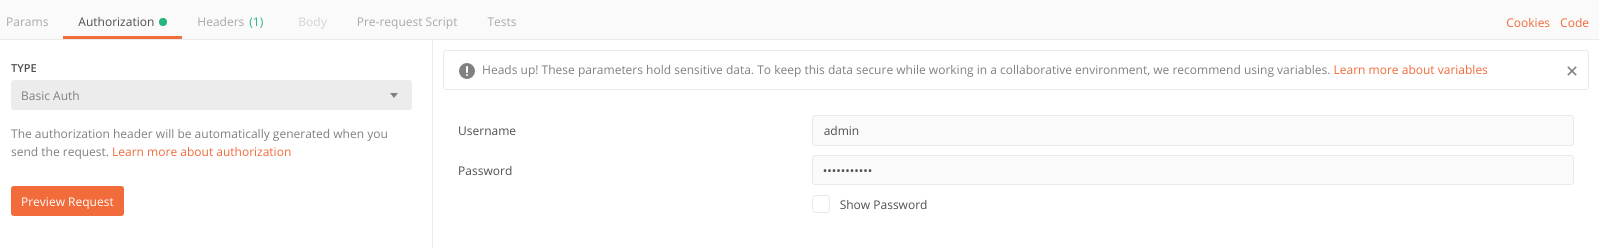
\includegraphics[width=\textwidth]
    {Technologien_Postman02}
    \caption{Postman GET Request}
    \label{fig:Postman}
\end{figure}


% HTTP und API müssen erklärt werden
\subsection{Kommunikation}
\label{sec:Kommunikation}
\subsubsection {Discord}
\label{sec:Discord}
Um im Laufe des praktischen Teils der Diplomarbeit die Übersicht zu behalten und alles zu organisieren wurde Discord verwendet. Discord hat viele Funktionen welche die Kommunikation im Team erleichtern. Discord bietet dem Benutzer an einen oder mehrere gratis Server zu erstellen. Ein Server kann aus Text und Sprachchannels bestehen. In einem Textchannel können festgelegte Personen schreiben und in einem Sprachchannel über Mikrofon miteinander reden. Falls wir also Teamintern etwas zu besprechen hatten oder falls Probleme auftraten die wir selbst lösen konnten bat Discord die perfekte Kommunikationsfläche. 

Da wir als Gruppe mehrere Projekte haben haben wir einen "Projektserver". In diesem Projektserver haben wir einen Text und Sprach Channel für die Diplomarbeit. Im Text Channel werden kleine Probleme, die schnell geklärt werden können, besprochen und Files ausgetauscht. Im Sprach Channel werden gröbere Probleme besprochen oder wenn nötig Planänderungen. 

%Installation und Server erstellung

\subsubsection {Telegram}
\label{sec:Telegram}
Telegram wurde nicht regelmäßig verwendet, es war eher eine Backup Chat-Application. 

\subsection{File Sharing}
\label{sec:FileSharing}
\subsubsection {TFS}
\label{sec:TFS}
Der Microsoft Team Foundation Server ist die verwendete Code-Sharing Technologie. Da der Auftraggeber, die Firma Intact GmbH oder Intact Systems, mit dieser Technologie arbeitet haben wir bei einem der ersten Treffer TFS für Code Sharing gewählt. Wir hatten einige Probleme mit dem TFS wodurch oft einzelne Teile des Projekts entwickelt wurden und dann in ein Projekt zusammengeführt wurden. Die Probleme waren unter anderem, dass die Firma eine Zeit lang gebraucht hat um den Server zur Verfügung zustellen aber auch, dass das Verbinden mit dem Server manchmal nicht geklappt hat. 

%Anleitung wie man einen TFS benutzt

\subsubsection {Discord}
\label{sec:Discord}
Wie bereits bei den Technologien erwähnt haben wir auf einem Discord Server einen Text Channel eingerichtet. Dieser eignet sich nicht nur um miteinander zu schreiben sondern kann auch dafür genutzt werden mit anderen Benutzer Files zu teilen. 
\subsubsection {Google Drive}
\label{sec:GoogleDrive}
Google Drive ist ein von Google bereitgestellter Cloud Service um Dokumente freizugeben, Online zu bearbeiten und zu speichern.

Mithilfe von Google Drive wurde an Präsentationen und Projekten gearbeitet. Durch Google Docs und Google Präsentation fällt es leicht mit mehreren Personen gleichzeitig an einem Dokument zu arbeiten. Durch Google Drive wurden Dokumente wie die IVM Matrix, den Projektstrukturplan, die Meetings und die SCRUM Sprints erstellt und an alle Mitglieder geteilt. 
\subsection{Organisation}
\label{sec:Organisation}
\subsubsection {Trello}
\label{sec:Trello}
Trello ist eine web-basiert Software die das managen von Projekten vereinfacht. Trello wurde benutzt um den management Prozess Scrum erfolgreich durchzuführen. Trello bietet eine gute Übersicht über den Status des Projekts, da es Aufgaben in Form von kleinen Karten in einer Liste anzeigt. Diese Aufgaben kann man mit einer Verantwortlichen Person inkl. Frist versehen. So wird dem Scrummaster die Möglichkeit geboten 3 Listen zu erstellen: ''To Do'', ''in Arbeit'' und ''Fertig''. Je nachdem in welchem Status sich die Aufgabe befindet wird sie dementsprechend zugeteilt.

\subsection{Schriftliche Arbeit}
\label{sec:TechSchriftlicheArbeit}
\subsubsection {LaTeX}
\label{sec:LaTeX}
LaTeX ist ein System mitdessen Hilfe man ein Dokument erstellen kann. Die Formatierung dieses Dokuments läuft anders als bei Word über Befehle. LaTeX läuft über das Textsatzsystem TeX. TeX hat seine eigene Sprache um Formatierungen von Text oder Grafiken sehr präzise und individuell einzustellen. 
\paragraph{Warum LaTeX?}
\label{sec:WarumLaTeX}
Warum wurde LaTeX verwendet und nicht Word oder sonstige Programme? Sobald bei einem Dokument vorgeschriebene Formatierung einzuhalten ist oder es einen großen Umfang haben wird, lohnt es sich LaTeX zu verwenden. Mit LaTeX werden Formatierung per Befehl definiert, man kann am Anfang des Dokuments gewisse Vorgaben definieren so kann man Standardmäßige Einstellungen vornehmen welche Formatierungsfehler beinahe komplett ausschließen. Nicht nur die Formatierung wird übersichtlicher und erleichtert, auch die Aufteilung des Projekts wird simpler. Es ist möglich ein Dokument als ''Haupt''-Dokument anzulegen und in diesem weitere einzelne Dokumente einzubinden. So kann man verschieden Themenbereiche in verschiedene Dokumente aufteilen. \cite{TechnologieLaTeX} 
\pagebreak